\subsubseccion{Ley Multinomial}
\label{Sssec:MP:Multinomial}

Esta ley es una generalizaci\'on de la ley binomial y aparece por ejemplo cuando
se  repite  una  experiencia  a  \  $k$  \ estados  \  $n$  \  veces  de  manera
independiente y nos  interesamos a la probabilidad que  el primer evento aparece
$n_1$ veces, el secundo $n_2$ veces, \ldots.  Se denota \ $X \ \sim \ \M(n,p)$ \
con  \  $n   \in  \Nset^*$  \  y   \  $p  =  \begin{bmatrix}  p_1   &  \cdots  &
  p_k  \end{bmatrix}^t \in  \Simp{k-1}$ \  the \  $(k-1)$-simplex  estandar (ver
figure~\ref{Fig:MP:Dirichlet}-(a)  y notaciones).  Entonces, a  pesar de  que se
escribe \  $X$ \ de manera  $k$-dimensional, el vector partenece  a una variedad
claramente \ $d = k-1$ \ dimensional y en el caso \ $k = 2$ \ se recupera la ley
binomial.  Las caracter\'isticas de \ $X \ \sim \ \M(n,p)$ \ son las siguientes:

\begin{caracteristicas}
%
Dominio de definici\'on~\footnote{De hecho, se puede considerar que el vector
aleatorio es \ $(k-1)$-dimensional \ $\widetilde{X} = \begin{bmatrix}
\widetilde{X}_1 & \cdots & \widetilde{X}_{k-1} \end{bmatrix}^t$ \ definido sobre
el dominio \ $\widetilde{\X} = \left\{ x \in \{ 0 \; \ldots \;
n\}^{k-1}, \: \sum_{i=1}^{k-1} x_i \le n
\right\}$.\label{Foot:MP:MultinomialDominio}} & $\X = \left\{ x \in \{ 0 \;
\ldots \; n\}^k, \: \sum_{i=1}^k x_i = n \right\}$\\[2mm]
\hline
%
Parametros & $n \in \Nset^*, \quad p \in  \Simp{k-1} = \left\{ p \in [ 0 \; 1
]^k, \: \sum_i p_i = 1 \right\}$\\[2mm]
\hline
%
Distribuci\'on de probabilidad~\footnote{Tratando de $\widetilde{X}$, su masa de
probabilidad es dada por \ $p_{\widetilde{X}}(x) = \frac{n!}{\prod_{i=1}^k x_i!}
\prod_{i=1}^{k-1} p_i^{x_i} \, \left( 1 - \sum_{i=1}^{k-1} p_i
\right)^{n-\sum_{i=1}^{k-1} x_i}$.\label{Foot:MP:MultinomialMasa}} &
$\displaystyle p_X(x) = \frac{n!}{\prod_{i=1}^k x_i!}  \prod_{i=1}^k
p_i^{x_i}$\\[2mm]
\hline
%
Promedio & $\displaystyle m_X = n \, p$\\[2mm]
\hline
%
Covarianza~\footnote{Fijense que, en este caso, $\Sigma_X \not\in P_k^+(\Rset)$
porque obviamente $\un^t \Sigma_Z \un = 0$. Es consecuencia directa del hecho de
que $X$ vive sobre $\Simp{k-1}$} & $\displaystyle \Sigma_X = n \left( \diag p -
p p^t \right)$\\[2mm]
\hline
%
Generadora de probabilidad & $\displaystyle G_X(z) = \left( p^t z
%\sum_{j=1}^k p_j z_j
\right)^n$ \ para \ $z \in \Cset^k$\\[2mm]
\hline
%
Generadora de momentos & \protect$\displaystyle M_X(u) = \left( p^t e^u
\right)^n, \: e^u = \begin{bmatrix} e^{u_1} & \cdots &
e^{u_k} \end{bmatrix}^t$\protect \ para \ $u \in \Cset^k$\\[2mm]
\hline
%
Funci\'on caracter\'istica & $\displaystyle \Phi_X(\omega) = \left( p^t e^{\imath \omega}
%\sum_{j=1}^k p_j e^{\imath \omega_j} 
\right)^n$
\end{caracteristicas}

% Momentos & $ \Esp\left[ X^k \right] = ??\\[2mm]
% Momento factorial & $\Esp\left[ (X)_k \right] = 
% \frac{(r+k-1)!}{(r-1)!} \left( \frac{p}{1-p} \right)^k$\\[2mm]
% Modo $\left\lfloor (n+1) p \right\rfloor$
% Mediana $\left\lfloor n p \right\rfloor$ o $\left\lceil n p \right\rceil
% CDF	$I_{1-p}(n-k,k+1)$ regularized incomplete beta function

\SZ{Agrecacion; corolario: Es sencillo  ver que  cada componente  \ $X_j$ \  es binomial,  $X_j \,  \sim \,
\B(n,p_j)$.}

Su masa  de probabilidad  y funci\'on de  repartici\'on son representadas  en la
figura Fig.~\ref{Fig:MP:Multinomial}.
%
\begin{figure}[h!]
\begin{center} 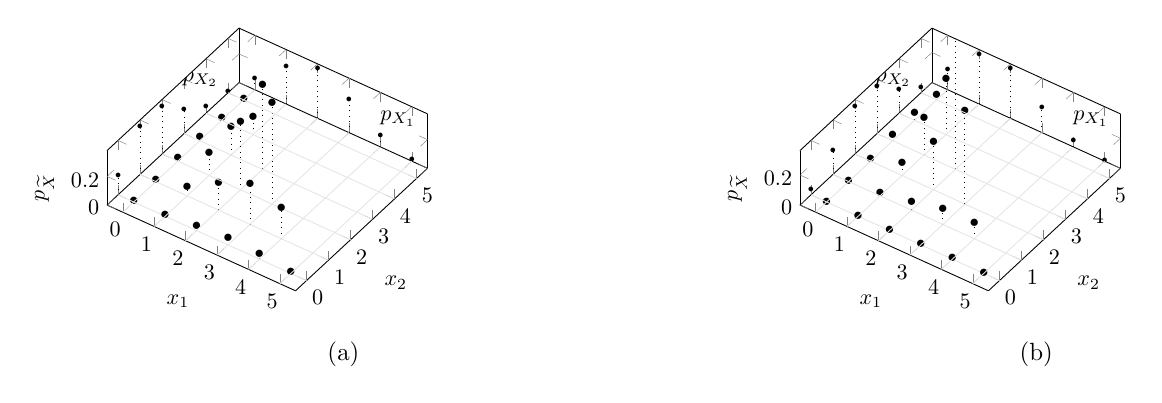
\begin{tikzpicture}[scale=.8]
\shorthandoff{>}
%
%
\pgfmathsetmacro{\n}{5};% numeros para la multinomial
\pgfmathsetmacro{\dec}{.5};% shitf para dibujar las marginales
%
% Ejemplo [6 5 4]/15
\begin{scope}
%
\pgfmathsetmacro{\pu}{2/5};% p_1
\pgfmathsetmacro{\pd}{1/3};% p_2
\pgfmathsetmacro{\qu}{floor((\n+1)*\pu)};% modo de la binomial 1
\pgfmathsetmacro{\qd}{floor((\n+1)*\pd)};% modo de la binomial 2
\pgfmathsetmacro{\mau}{factorial(\n)/factorial(\qu)/factorial(\n-\qu)*(\pu^\qu)*((1-\pu)^(\n-\qu))};% maximo de la binomial 1
\pgfmathsetmacro{\mad}{factorial(\n)/factorial(\qd)/factorial(\n-\qd)*(\pd^\qd)*((1-\pd)^(\n-\qd))};% maximo de la binomial 2
\pgfmathsetmacro{\ma}{max(\mau,\mad)};% maximo de ambas binomiales
%
\begin{axis}[
    colormap = {whiteblack}{color(0cm)  = (white);color(1cm) = (black)},
    width=.55\textwidth,
    view={35}{70},
    enlargelimits=false,
    xmin={-\dec},
    xmax={\n+\dec},
    ymin={-\dec},
    ymax={\n+\dec},
    zmax={1.1*\ma},
    color=black,
    xtick={0,...,\n},
    ytick={0,...,\n},
    xlabel=$x_1$,
    ylabel=$x_2$,
    zlabel=$p_{\widetilde{X}}$,
]
%
\pgfmathsetmacro{\bu}{(1-\pu-\pd)^\n};% coeficiente binomial por la probabilidad p1
\pgfmathsetmacro{\bd}{\bu};% coeficiente binomial por la probabilidad p2
%
\pgfmathsetmacro{\bmu}{(1-\pu)^\n};% lo mismo para la marginale 1
\pgfmathsetmacro{\bmd}{(1-\pd)^\n};% lo mismo para la marginale 2
%
\foreach \mu in {0,...,\n} {
  \foreach \md in {0,...,\n} {
    \ifnum \numexpr\mu+\md < \numexpr\n+1
      \addplot3 [dotted,domain=0:\bd,samples=2, samples y=0,color=black] (\mu,\md,\x)  node[scale=.85]{$\bullet$};
      %
      \pgfmathsetmacro{\bld}{\bd*\pd*(\n-\md)/((\md+1)*(1-\pu-\pd))};
      \global\let\bd\bld;% proba en m2 (m1 fijo) actualizado
    \fi
  }
  %
  % Marginales
  \addplot3 [dotted,domain=0:\bmu,samples=2, samples y=0,color=black] (\mu,{\n+\dec},\x)  node[scale=.55]{$\bullet$};
  \addplot3 [dotted,domain=0:\bmd,samples=2, samples y=0,color=black] ({-\dec},\mu,\x)  node[scale=.55]{$\bullet$};
  %
  % lineas (m1,m2) abajo
  \addplot3 [domain={-\dec}:{\n+\dec},samples=2, samples y=0,color=black!10] (\mu,\x,0);
  \addplot3 [domain={-\dec}:{\n+\dec},samples=2, samples y=0,color=black!10] (\x,\mu,0);
  %
  \pgfmathsetmacro{\blu}{\bu*\pu*(\n-\mu)/((\mu+1)*(1-\pu-\pd))};
  \global\let\bu\blu;\global\let\bd\blu;% proba inicial en m1 actualizada
  %
  % lo mismo para cada marginal
  \pgfmathsetmacro{\blmu}{\bmu*\pu*(\n-\mu)/((\mu+1)*(1-\pu))};
  \global\let\bmu\blmu;% proba 1 actualizada
  \pgfmathsetmacro{\blmd}{\bmd*\pd*(\n-\mu)/((\mu+1)*(1-\pd))};
  \global\let\bmd\blmd;% proba 2 actualizada
}
%
\node at (axis cs:{3*\n/4},{\n+\dec},{\mau/2})[right]{$p_{X_1}$};
\node at (axis cs:{-\dec},{3*\n/4},{\mad/2})[above]{$p_{X_2}$};
\end{axis}
\node at ({3*\n/4},-1)[scale=.9]{(a)};
\end{scope}
%
%
%
%
% Ejemplo [1 1 1]/3
\begin{scope}[xshift = 11cm]
%
\pgfmathsetmacro{\pu}{1/3};% p_1
\pgfmathsetmacro{\pd}{1/2};% p_2
\pgfmathsetmacro{\qu}{floor((\n+1)*\pu)};% modo de la binomial 1
\pgfmathsetmacro{\qd}{floor((\n+1)*\pd)};% modo de la binomial 2
\pgfmathsetmacro{\mau}{factorial(\n)/factorial(\qu)/factorial(\n-\qu)*(\pu^\qu)*((1-\pu)^(\n-\qu))};% maximo de la binomial 1
\pgfmathsetmacro{\mad}{factorial(\n)/factorial(\qd)/factorial(\n-\qd)*(\pd^\qd)*((1-\pd)^(\n-\qd))};% maximo de la binomial 2
\pgfmathsetmacro{\ma}{max(\mau,\mad)};% maximo de ambas binomiales
%
\begin{axis}[
    colormap = {whiteblack}{color(0cm)  = (white);color(1cm) = (black)},
    width=.55\textwidth,
    view={35}{70},
    enlargelimits=false,
    xmin={-\dec},
    xmax={\n+\dec},
    ymin={-\dec},
    ymax={\n+\dec},
    zmax={1.1*\ma},
    color=black,
    xtick={0,...,\n},
    ytick={0,...,\n},
    xlabel=$x_1$,
    ylabel=$x_2$,
    zlabel=$p_{\widetilde{X}}$,
]
%
\pgfmathsetmacro{\bu}{(1-\pu-\pd)^\n};% coeficiente binomial por la probabilidad p1
\pgfmathsetmacro{\bd}{\bu};% coeficiente binomial por la probabilidad p2
%
\pgfmathsetmacro{\bmu}{(1-\pu)^\n};% lo mismo para la marginale 1
\pgfmathsetmacro{\bmd}{(1-\pd)^\n};% lo mismo para la marginale 2
%
\foreach \mu in {0,...,\n} {
  \foreach \md in {0,...,\n} {
    \ifnum \numexpr\mu+\md < \numexpr\n+1
      \addplot3 [dotted,domain=0:\bd,samples=2, samples y=0,color=black] (\mu,\md,\x)  node[scale=.85]{$\bullet$};
      %
      \pgfmathsetmacro{\bld}{\bd*\pd*(\n-\md)/((\md+1)*(1-\pu-\pd))};
      \global\let\bd\bld;% proba en m2 (m1 fijo) actualizado
    \fi
  }
  %
  % Marginales
  \addplot3 [dotted,domain=0:\bmu,samples=2, samples y=0,color=black] (\mu,{\n+\dec},\x)  node[scale=.55]{$\bullet$};
  \addplot3 [dotted,domain=0:\bmd,samples=2, samples y=0,color=black] ({-\dec},\mu,\x)  node[scale=.55]{$\bullet$};
  %
  % lineas (m1,m2) abajo
  \addplot3 [domain={-\dec}:{\n+\dec},samples=2, samples y=0,color=black!10] (\mu,\x,0);
  \addplot3 [domain={-\dec}:{\n+\dec},samples=2, samples y=0,color=black!10] (\x,\mu,0);
  %
  \pgfmathsetmacro{\blu}{\bu*\pu*(\n-\mu)/((\mu+1)*(1-\pu-\pd))};
  \global\let\bu\blu;\global\let\bd\blu;% proba inicial en m1 actualizada
  %
  % lo mismo para cada marginal
  \pgfmathsetmacro{\blmu}{\bmu*\pu*(\n-\mu)/((\mu+1)*(1-\pu))};
  \global\let\bmu\blmu;% proba 1 actualizada
  \pgfmathsetmacro{\blmd}{\bmd*\pd*(\n-\mu)/((\mu+1)*(1-\pd))};
  \global\let\bmd\blmd;% proba 2 actualizada
}
%
\node at (axis cs:{3*\n/4},{\n+\dec},{\mau/2})[right]{$p_{X_1}$};
\node at (axis cs:{-\dec},{3*\n/4},{\mad/2})[above]{$p_{X_2}$};
\end{axis}
\node at ({3*\n/4},-1)[scale=.9]{(b)};
\end{scope}
%
\end{tikzpicture} \end{center}
%
\leyenda{Ilustraci\'on de una distribuci\'on  de probabilidad multinomial para \
  $k   =  3$   \   del   vector  \   $(k-1)$-dimensional   \  $\widetilde{X}   =
  \protect\begin{bmatrix}   X_1  &  X_2   \protect\end{bmatrix}^t$  \   ($X_3  =
  1-X_1-X_2$)  \ con  las marginales  \ $p_{X_1},  \: p_{X_2}$  \ (ver  notas de
  pie~\ref{Foot:MP:MultinomialDominio}   y~\ref{Foot:MP:MultinomialMasa}).   Los
  otros parametros son  \ $n = 5$  \ y \ $p =  \protect\begin{bmatrix} \frac25 &
    \frac13     &    \frac4{15}     \protect\end{bmatrix}^t$    (a),     $p    =
  \protect\begin{bmatrix} \frac13  & \frac12 &  \frac16 \protect\end{bmatrix}^t$
  (b).}
\label{Fig:MP:Multinomial}
\end{figure}


\SZ{Otros ilustraciones para otros $n, p$?}